%%%%%%%%%%%%%%%%%%%%%%%%%%%%%%%%%%%%%%%%%%%%%%%%%%%%%%%%%%%%%%%%%%%%
%%%           Vorlage für eine Ausarbeitung an der DHBW          %%%
%%%                                                              %%%
%%%      Bereiche die bearbeitet werden müssen werden durch      %%%
%%%      einen solchen Kommentarblock eingeleitet und enden      %%%
%%%      mit der nächsten Trennlinie.                            %%%
%%%                                                              %%%
%%%      In dieser Datei müssen folgende Bereiche bearbeitet     %%%
%%%      werden:                                                 %%%
%%%      - Angaben zur Arbeit                                    %%%
%%%      - EIGENE KAPITEL EINFÜGEN                               %%%
%%%                                                              %%%
%%%      Benötigte Seiten und Verzeichnisse können unter         %%%
%%%      "Einführung und Verzeichnisse" ein- bzw. auskommentiert %%%
%%%      werden.                                                 %%%
%%%                                                              %%%
%%%%%%%%%%%%%%%%%%%%%%%%%%%%%%%%%%%%%%%%%%%%%%%%%%%%%%%%%%%%%%%%%%%%

\documentclass[a4paper,12pt]{article}
\usepackage[left=2.5cm,right=2.5cm,top=2.5cm,bottom=2.5cm,includehead]{geometry}      % Einstellungen der Seitenränder
\usepackage[english, ngerman]{babel}                                                  % deutsche Silbentrennung
\usepackage[utf8]{inputenc}                                                           % Umlaute
\usepackage[T1]{fontenc}													                                    % Umlaute auch richtig ausgeben
\usepackage{newtxtext,newtxmath}                                                      % Font = Times New Roman
\usepackage{hyperref}
\usepackage[nottoc]{tocbibind}
\usepackage{fancyhdr}
\usepackage{setspace}
\usepackage[backend=bibtex, citestyle=authoryear, bibstyle=authoryear]{biblatex}      % Bibliothek für Zitate
\usepackage{csquotes}                                                                 % Zusatzpacket für Zitate
\usepackage{amsmath}                                                                  % Zurücksetzen der Tabellen- und Abbildungsnummerierung je Sektion
\usepackage[labelfont=bf,aboveskip=1mm]{caption}                                      % Bild- und Tabellenunterschrift (fett)
\usepackage[bottom,multiple,hang,marginal]{footmisc}                                  % Fußnoten [Ausrichtung unten, Trennung durch Seperator bei mehreren Fußnoten]
\usepackage{graphicx}  
\graphicspath{{./images/}}                                                            % Grafiken
\usepackage[dvipsnames]{xcolor}                                                       % Farbige Buchstaben
\usepackage{wrapfig}                                                                  % Bilder in Text integrieren
\usepackage{enumitem}                                                                 % Befehl setlist (Zeilenabstand für itemize Umgebung auf 1 setzen)
\usepackage{listings}                                                                 % Quelltexte
\definecolor{commentgreen}{RGB}{87,166,74}                                            % Kommentar-Farbe für Quellcode
\lstset{numbers=left, numberstyle=\tiny, numbersep=8pt, frame=single, framexleftmargin=15pt, breaklines=true, commentstyle=\color{commentgreen}}
\usepackage{tabularx}                                                                 % Tabellen
\usepackage{multirow}                                                                 % Mehrzeilige Tabelleneinträge
\usepackage[addtotoc]{abstract}                                                       % Abstract
\usepackage[nohyperlinks, printonlyused, withpage]{acronym}                           % Abkürzungen
\usepackage{dirtree}                                                                  % Ordnerstruktur (z.B. für Anhang)
\usepackage{float}
\usepackage{pdfpages}

%%%%%%%%%%%%%%%%%%%%%%%%%%%%%%%%%%%%%%%%%%%%%%%%%%%%%%%%%%%%%%%%%%%%
%%%                      Angaben zur Arbeit                      %%%
%%%%%%%%%%%%%%%%%%%%%%%%%%%%%%%%%%%%%%%%%%%%%%%%%%%%%%%%%%%%%%%%%%%%
\def\vFirmenlogoPfad{}                  %% relativer Pfad Bsp.: images/Firmenlogo.png
\def\vDHBWLogoPfad{images/DHBW_logo.jpg}                          %% relativer Pfad Bsp.: images/DHBW_logo.jpg
\def\vUnterschrift{}                    %% Pfad zu Bild mit Unterschrift (für digitale Abgabe) Bsp.: images/Unterschrift.png

\def\vTitel{Softwarequalität}                           %% 
\def\vUntertitel{}                      %% 
\def\vArbeitstyp{Hausarbeit}                      %% Projektarbeit/Seminararbeit/Bachelorarbeit
\def\vArbeitsbezeichnung{}              %% T1000/T2000/T3000

\def\vLB{Lukas Braun}
\def\vJB{Johannes Brandenburger}
\def\vHS{Henry Schuler}
\def\vPP{Phillipp Patzelt}


\def\vAutor{\vJB, \vLB, \vPP, \vHS}                           %% Vorname Nachname
\def\vMatrikelnummer{}                  %% 7-stellige Zahl
\def\vKursKuerzel{TIT20}                     %% Bsp.: TIT20
\def\vPhasenbezeichnung{Theoriephasen}               %% Praxisphase/Theoriephase
\def\vStudienJahr{dritte}                     %% erste/zweite/dritte
\def\vDHBWStandort{Ravensburg}                    %% Bsp.: Ravensburg
\def\vDHBWCampus{Friedrichshafen}                      %% Bsp.: Friedrichshafen
\def\vFakultaet{Technik}                       %% Technik/Wirtschaft
\def\vStudiengang{Informatik}                     %% Informationstechnik/...
\def\vKurs{TIT20}                     %% IT/...

\def\vBearbeitungsort{Friedrichshafen}                 %%                       %% 
\def\vBetreuer{Benjamin Jung}                        %% Vorname Nachname

\def\vAbgabedatum{\today}               %% DD. MONTH YYYY
\def\vBearbeitungszeitraum{01.10.2022 - 06.01.2023}            %% DD.MM.YYYY - DD.MM.YYYY
%TODO Datum anpassen

%%%%%%%%%%%%%%%%%%%%%%%%% Eigene Kommandos %%%%%%%%%%%%%%%%%%%%%%%%%
% Definition von \gqq{}: Text in Anführungszeichen
\newcommand{\gqq}[1]{\glqq #1\grqq}
% Definition von \gq{}: Text in Anführungszeichen
\newcommand{\gq}[1]{\glq #1\grq}
% Spezielle Hervorhebung von Schlüsselwörtern
\newcommand{\textOrdner}[1]{\texttt{#1}}
\newcommand{\textVariable}[1]{\texttt{#1}}
\newcommand{\textKlasse}[1]{\texttt{#1}}
\newcommand{\textFunktion}[1]{\texttt{#1}}
\newcommand{\newparagraph}{\newline \newline}
% Quellenangabe bei Bildern
\newcommand{\customcaption}[2]{\caption[#1]{ #1. #2.}}

%%%%%%%%%%%%%%%%%%%% Zitatbibliothek einbinden %%%%%%%%%%%%%%%%%%%%%
\addbibresource{./literatur/literatur.bib}


%%%%%%%%%%%%%%%%%%%%%%%% PDF-Einstellungen %%%%%%%%%%%%%%%%%%%%%%%%%
\hypersetup{
  bookmarksopen=false,
	bookmarksnumbered=true,
	bookmarksopenlevel=0,
  pdftitle=\vTitel,
  pdfsubject=\vTitel,
  pdfauthor=\vAutor,
  pdfborder={0 0 0},
	pdfstartview=Fit,
  pdfpagelayout=SinglePage
}


%%%%%%%%%%%%%%%%%%%%%%%% Kopf- und Fußzeile %%%%%%%%%%%%%%%%%%%%%%%%
\pagestyle{fancy}
\setlength{\headheight}{15pt}
\fancyhf{}
\fancyhead[R]{\thepage}


%%%%%%%%%%%%%%%%%%%%%%%%%%%%%% Layout %%%%%%%%%%%%%%%%%%%%%%%%%%%%%%
\onehalfspacing
\setlist{noitemsep}

\addto\captionsngerman{
  \renewcommand{\figurename}{Abb.}
  \renewcommand{\tablename}{Tab.}
}
\numberwithin{table}{section}                               % Tabellennummerierung je Sektion zurücksetzen
\numberwithin{figure}{section}                              % Abbildungsnummerierung je Sektion zurücksetzen
\renewcommand{\thetable}{\arabic{section}.\arabic{table}}   % Tabellennummerierung mit Section
\renewcommand{\thefigure}{\arabic{section}.\arabic{figure}} % Abbildungsnummerierung mit Section
\renewcommand{\thefootnote}{\arabic{footnote}}              % Sektionsbezeichnung von Fußnoten entfernen

\renewcommand{\multfootsep}{, }                             % Mehrere Fußnoten durch ", " trennen


%%%%%%%%%%%%%%%%%%%%%%%%%%%%% Dokument %%%%%%%%%%%%%%%%%%%%%%%%%%%%%

\begin{document}


  %%%%%%%%%%%%%%%%%%% Einführung und Verzeichnisse %%%%%%%%%%%%%%%%%%%
  \pagenumbering{Roman}

  \begin{titlepage}
  \begin{minipage}{6in}
    \vspace*{-2cm}
    \centering
    \hspace{-2cm}
	\ifx\vFirmenlogoPfad\empty
	\else
    \raisebox{-0.5\height}{\includegraphics[height=4cm]{\vFirmenlogoPfad}}
  \fi
	\hfill
	\ifx\vDHBWLogoPfad\empty
	\else
   	\raisebox{-0.5\height}{\includegraphics[height=4cm]{\vDHBWLogoPfad}}
	\fi
  \end{minipage}
  \begin{center}
    \vspace*{0.5cm}
    \Huge\textbf{\vTitel}\\
		\ifx\vUntertitel\empty
		\else
			\Large\rm\vUntertitel\\
		\fi
		\vspace*{2cm}
		\Large\textbf{\vArbeitstyp}
		\ifx\vArbeitsbezeichnung\empty
		\else
			\textbf{\vArbeitsbezeichnung}
		\fi
		\\
		\normalsize
		über die \vPhasenbezeichnung\ des \vStudienJahr{n}\ Studienjahrs \\
		\vspace*{1cm}
		an der Fakultät für \vFakultaet\\
		im Studiengang \vStudiengang\\
		\vspace*{0.5cm}
		an der DHBW \vDHBWStandort\\
		\ifx\vDHBWCampus\empty
		\else
		Campus \vDHBWCampus\\
		\fi
		\vspace*{0.5cm}
		von\\
		\ifx\vAutor\empty
		\else
			\vAutor\\
		\fi
		\vspace*{1cm}
		\vAbgabedatum
		\vfill
  \end{center}
  \begin{tabular}{ll}
    Bearbeitungszeitraum:&\vBearbeitungszeitraum\\
    Kurs:&\vKurs\\
	  Dozent der Hochschule:&\vBetreuer\\
  \end{tabular}
\end{titlepage}
\newpage
\setcounter{page}{2}
  % \thispagestyle{empty}
\section*{\Huge{Sperrvermerk}}

\addcontentsline{toc}{section}{Sperrvermerk}
gemäß Ziffer 1.1.13 der Anlage 1 zu §§ 3, 4 und 5  der Studien- und Prüfungsordnung für die Bachelorstudiengänge im Studienbereich Technik der Dualen Hochschule Baden-Würt­tem­berg vom 29.09.2017.\\

\noindent \gqq{Der Inhalt dieser Arbeit darf weder als Ganzes noch in Auszügen Personen außerhalb des Prüfungsprozesses und des Evaluationsverfahrens zugänglich gemacht werden, sofern keine anders lautende Genehmigung vom Dualen Partner vorliegt.}

\vfill
\leavevmode
\newline
\parbox{6cm}{\strut\centering \vBearbeitungsort, \vAbgabedatum\hrule\strut\centering\footnotesize Ort, Datum} 
\hfill
\ifx\vUnterschrift\empty
\parbox{6cm}{\strut\hspace{1pt} \vAbteilung\hrule\strut\centering\footnotesize Abteilung, Unterschrift}
\else
\parbox{6cm}{\strut\hspace{1pt} \vAbteilung, \parbox[b]{3cm}{\vspace{-10cm}\includegraphics[width=3cm]{\vUnterschrift}}\hrule\strut\centering\footnotesize Abteilung, Unterschrift}
\fi
\vspace{1cm}

\newpage
  \thispagestyle{empty}
\section*{\Huge{Gender Erklärung}}

\addcontentsline{toc}{section}{Gendererklärung}
Aus Gründen der besseren Lesbarkeit wird in dieser Bachelorarbeit auf die gleichzeitige Verwendung der Sprachformen männlich,
weiblich und divers (m/w/d) verzichtet. Sämtliche Formulierungen gelten gleichermaßen für alle Geschlechter.
\newpage
  \thispagestyle{empty}
\section*{\Huge{Selbstständigkeitserklärung}}

\addcontentsline{toc}{section}{Selbstständigkeitserklärung}
gemäß Ziffer 1.1.13 der Anlage 1 zu §§ 3, 4 und 5  der Studien- und Prüfungsordnung für die Bachelorstudiengänge im Studienbereich Technik der Dualen Hochschule Baden-Würt­tem­berg vom 29.09.2017.

\noindent Wir versichern hiermit, dass wir unsere Bachelorarbeit (bzw. Projektarbeit oder Studienarbeit bzw. Hausarbeit) mit dem Thema: 
\begin{center}
	\Large\textbf{\vTitel}
\end{center}
selbstständig verfasst und keine anderen als die angegebenen Quellen und Hilfsmittel benutzt haben. Wir versichern zudem, dass die eingereichte elektronische Fassung mit der gedruckten Fassung übereinstimmt.

\vfill
\leavevmode
\newline
\parbox{7cm}{\strut\centering \vBearbeitungsort, \vAbgabedatum\hrule\strut\centering\footnotesize Ort, Datum} 
\hfill
\parbox{7cm}{\strut\hspace{1pt} \hrule\strut\centering\footnotesize \vJB}
\newline
\vspace{1cm}
\newline
\parbox{7cm}{\strut\centering \vBearbeitungsort, \vAbgabedatum\hrule\strut\centering\footnotesize Ort, Datum} 
\hfill
\parbox{7cm}{\strut\hspace{1pt} \hrule\strut\centering\footnotesize \vLB}
\newline
\vspace{1cm}
\newline
\parbox{7cm}{\strut\centering \vBearbeitungsort, \vAbgabedatum\hrule\strut\centering\footnotesize Ort, Datum} 
\hfill
\parbox{7cm}{\strut\hspace{1pt} \hrule\strut\centering\footnotesize \vPP}
\newline
\vspace{1cm}
\newline
\parbox{7cm}{\strut\centering \vBearbeitungsort, \vAbgabedatum\hrule\strut\centering\footnotesize Ort, Datum} 
\hfill
\parbox{7cm}{\strut\hspace{1pt} \hrule\strut\centering\footnotesize \vHS}
\newpage
  %\phantomsection
\newenvironment{keywords}{
	\begin{flushleft}
	\small	
	\textbf{
		\iflanguage{ngerman}{Schlüsselwörter}{\iflanguage{english}{Keywords}{}}
	}
}{\end{flushleft}}

% Deutsche Zusammenfassung
\begin{abstract}
	
\end{abstract}

% Schlüsselwörter Deutsch
\begin{keywords}
	
\end{keywords}


\selectlanguage{english}
% Englisches Abstract
\begin{abstract}

\end{abstract}

% Schlüsselwörter Englisch
\begin{keywords}

\end{keywords}


\selectlanguage{ngerman}
\newpage
  \pdfbookmark[1]{\contentsname}{toc}
\tableofcontents
\newpage
  \section*{Abkürzungsverzeichnis}
\addcontentsline{toc}{section}{Abkürzungsverzeichnis}
\begin{acronym}
  \acro{DHBW}[DHBW]{Duale Hochschule Ba\-den-\-Würt\-tem\-berg}
  \acroplural{DHBW}[DHBW]{Dualen Hochschule Ba\-den-\-Würt\-tem\-berg}
  \acro{ISO}[ISO]{International Organization for Standardization}
  \acro{RE}[RE]{Requirements Engineering}
  \acro{FMEA}[FMEA]{Failure Mode and Effects Analysis}
  \acro{KVP}[KVP]{Kontinuierlicher Verbesserungs Prozess}
  \acro{CMMI}[CMMI]{Capability Maturity Model Integration}
\end{acronym}
\newpage
  \listoffigures
\newpage
  \listoftables
\newpage
  \lstlistoflistings
\addcontentsline{toc}{section}{Listings}
\newpage
  % \section*{Vorwort}
\addcontentsline{toc}{section}{Vorwort}
\newpage


  %%%%%%%%%%%%%%%%%%%%%%%%%%%%% Kapitel %%%%%%%%%%%%%%%%%%%%%%%%%%%%%%
  \pagestyle{fancy}
  \fancyhead[L]{\nouppercase{\rightmark}}    % Abschnittsname im Header
  \pagenumbering{arabic}

  %%%%%%%%%%%%%%%%%%%%%%%%%%%%%%%%%%%%%%%%%%%%%%%%%%%%%%%%%%%%%%%%%%%%
  %%%%                   EIGENE KAPITEL EINFÜGEN                  %%%%
  %%%%%%%%%%%%%%%%%%%%%%%%%%%%%%%%%%%%%%%%%%%%%%%%%%%%%%%%%%%%%%%%%%%%
  \section{Einleitung}
Die Hausarbeit wird im Rahmen der Vorlesung Softwarequalität erstellt.
Dabei werden zunächst Grundwissen und Begriffe definiert, anschließend werden die erlernten Fähigkeiten auf eine konkretes Produkt angewandt.
Hierzu wird das Softwareprodukt \gqq{DEV-CHAT} aus der Vorlesung Software Engineering 1 verwendet.
\newparagraph
%Beschreibung devchat
DEV-CHAT ist ein Chatportal mit mehreren Chatrooms, denen man über einen Schlüssel beitreten kann.
Die Oberfläche ist schlicht im Informatik/Konsolen Stil gehalten und alle Operationen werden über eine Kommandozeile ausgeführt.
Über die Kommandozeile lassen sich Befehle ausführen, um zum Beispiel Direktnachrichten zu senden oder Umfragen zu starten.
\newparagraph
%Aufgabenstellung
Zu Begin der Hausarbeit werden, wie bereits angekündigt, die Begriffe Softwarequalität und Qualität definiert und gegeneinander abgegrenzt, anschließend wird das Kano-Modell erläutert und begründet wieso Requirements Engineering essenziell für eine hohe Softwarequalität ist.
Die Folgeschritte werden auf den DEV-CHAT angewandt, diese gliedern sich in drei Punkte.
Zunächst werden die Anforderungen und Nutzerwartungen definiert, in einem weiteren Schritt werden Fehler, Kosten und Qualitätsmaßnahmen behandelt.
Abschließend wird das Thema Umsetzung und Tests erörtert.
  \section{Grundwissen und Begriffe}
In diesem Kapitel werden die Grundlegenden Begriffe und Konzepte vorgestellt und erläutert.
Dazu wird zunächst der generische Begriff der Qualität definiert und anschließend gegenüber der Software-Qualität abgegrenzt.
Weiterhin wird das Kano-Modell vorgestellt und dessen Bedeutung in Zusammenhang mit dem Requirements Engineering in Bezug auf die Software-Qualität erläutert.
\subsection{Qualität}
Der Begriff Qualität leitet sich von dem lateinischen Begriff \gqq{qualitas} ab, welcher mit den Begriffen \gqq{Beschaffenheit} oder \gqq{Eigenschaft} übersetzt werden kann \autocite[vgl.][]{noauthor_was_nodate}.
Die \ac{ISO} beschreibt den Begriff Qualität als \gqq{Grad, in dem ein Satz inhärenter Merkmale eines Objekts Anforderungen erfüllt} \autocite[S. 17]{iso_iso_2015}.
Die Merkmale, sowie Anforderungen des Objekts werden dabei nicht weiter konkretisiert.
Es handelt sich also um Aspekte, welche nicht universell definiert werden können.
Qualität ist somit ein sehr abstrakter Begriff, welcher je nach Kontext unterschiedlich interpretiert werden kann.

Um eine Aussage über die Qualität eines Objekts tätigen und mit anderen Objekten vergleichen zu können, muss Qualität messbar gemacht werden.
Dafür müssen zunächst die wesentlichen gemeinsamen Merkmale definiert werden.
In einem weiteren Schritt muss dann eine Art und Weise gefunden werden, wie diese spezifischen Merkmale hinsichtlich ihres Umsetzungsgrades bewertet werden können.
Die Bewertung kann dabei sowohl subjektiv als auch objektiv erfolgen \autocite[vgl.][S. 53]{shewhart_economic_1931}.
Das Merkmal Benutzerfreundlichkeit kann beispielsweise durch die Auswertung verschiedener subjektiver Eindrücke von Test-Benutzer bestimmt werden.
Gleichzeitig kann aber auch eine objektive Bewertung vorgenommen werden, indem beispielsweise Faktoren wie die Anzahl an Funktionen zusammen mit der Komplexität der einzelnen Funktionen des Objekts gemessen werden.

\subsection{Software-Qualität}
Der Begriff Software-Qualität stellt eine Spezifizierung des Begriffs Qualität dar, indem der Begriff Qualität in den Kontext Software gestellt wird.
Durch diese Spezifizierung konkretisiert sich auch die Definition des Begriffs (Software-)Qualität, welcher als "Grad, in dem ein Softwareprodukt festgelegte und implizierte Anforderungen erfüllt, wenn es unter bestimmten Bedingungen verwendet wird" \autocite[S. 17]{iso_iso_2011}, definiert werden kann.
Die wesentlichen Merkmale für die Bewertung der Qualität von Software unterteilen sich dabei in zwei Gruppen -- die externe und die interne Qualitätssicht.

Die externe Qualitätssicht bezieht sich auf Software-Merkmale, welche für die anwendende Person die Qualität der Software beeinflusst.
Dazu zählen die vier Merkmale Funktionalität, Laufzeit, Zuverlässigkeit und Benutzbarkeit.

Auf der anderen Seite steht die interne Qualitätssicht, welche sich auf Software-Merkmale, welche für die entwickelnde Person relevant sind, bezieht.
Dazu zählen die Merkmale Wartbarkeit, Transparenz, Übertragbarkeit sowie Testbarkeit \autocite[vgl.][S. 6-10]{hoffmann_software-qualitat_2013}.

\subsection{Kano-Modell}
Damit ein entwickeltes Produkt einen möglichst hohen Gewinn generieren kann, muss das Produkt möglichst oft abgesetzt werden können.
Dies kann unter anderem durch eine Steigerung der Kundenzufriedenheit erreicht werden.
Um diese systematisch zu erreichen, entwickelte der japanische Professor Noriaki Kano in den 70er Jahren das Kano-Modell \autocite[vgl.][S. 27]{sauerwein_kano-modell_2000}.
Kano definiert dafür fünf Kategorien, in welche sich die Merkmale eines Produktes einteilen lassen: 
Basismerkmale (Must-be quality elements), Leistungsmerkmale (One-dimensional quality elements), Begeisterungsmerkmale (Attractive quality elements), Unerhebliche-Merkmale (Indifferent quality elements) und Rückweisungsmerkmale (Reverse quality elements) \autocite[vgl.][S. 82-83]{holzing_kano-theorie_2008}.

\begin{figure}
  \centering
  \includegraphics[width=0.8\textwidth, keepaspectratio]{images/kano-modell.png}
  \caption{Kano-Modell \autocite{diehl_kano_2019}}
  \label{fig:kano-modell}
\end{figure}
Die einzelnen Kategorien unterscheiden sich hinsichtlich ihrer Wirkung auf die Kundenzufriedenheit.
Abbildung~\ref{fig:kano-modell} zeigt drei der fünf Kategorien des Kano-Modells.
Die x-Achse definiert dabei den Grad der Erfüllung der Merkmale, wobei die y-Achse den Grad der Kundenzufriedenheit darstellt.

Die rote Kurve in Abbildung~\ref{fig:kano-modell} zeigt die Charakteristik der Basismerkmale.
Während eine unzureichende Erfüllung des Merkmals zu einer negativen Kundenzufriedenheit führt, führt eine übermäßige Erfüllung des Merkmals nicht zu einer positiven Kundenzufriedenheit, da diese Merkmale als absolutes Minimum (Must-be) angesehen werden.

Im Gegensatz dazu stehen die Leistungsmerkmale, welche durch die blaue Kurve charakterisiert werden.
Hierbei handelt es sich um einen linearen Zusammenhang zwischen dem Grad der Erfüllung eines Merkmals und der Kundenzufriedenheit.
Durch Erfüllung dieser Merkmale kann somit im Gegensatz zu den Basismerkmalen die Kundenzufriedenheit gesteigert werden.

Begeisterungsmerkmale stellen das Komplement zu den Basismerkmalen dar und sind in Abbildung~\ref{fig:kano-modell} durch die rosa Kurve dargestellt.
Dabei handelt es sich um optionale Merkmale, welche die Kundenzufriedenheit ausschließlich steigern können.
Werden die Merkmale nicht erfüllt beeinflusst dies die Kundenzufriedenheit somit weder positiv noch negativ.

Neben den drei eingezeichneten Kurven in Abbildung~\ref{fig:kano-modell} wird die Klasse der Unerheblichen-Merkmale durch die x-Achse charakterisiert.
Diese Merkmale sind für die Kundenzufriedenheit nicht relevant, da sie diese weder positiv noch negativ beeinflussen.

Die letzte Klasse, die Rückweisungsmerkmale, stellen das Komplement zu den Leistungsmerkmalen dar.
Es besteht somit ebenfalls ein linearer Zusammenhang zwischen dem Grad der Erfüllung eines Merkmals und der Kundenzufriedenheit, jedoch in umgekehrter Richtung.
In Abbildung~\ref{fig:kano-modell} würde diese Klasse der blauen Geraden entsprechen, welche um 90 Grad im Ursprung gedreht wurde.
Bei nicht Erfüllung des Merkmals wird somit eine hohe Kundenzufriedenheit hervorgerufen, wohingegen eine Erfüllung des Merkmals die Kundenzufriedenheit negativ beeinflusst.
\newline

% TODO: @Henry Zusammenhang Qualität und Kano-Modell ?

\subsection{Requirements Engineering}
\ac{RE} ist ein Teilgebiet der Software-Entwicklung, welches sich mit der Erhebung, Analyse und Spezifikation von Anforderungen an ein Software-Produkt befasst.
Diese Anforderungen werden dabei durch die Stakeholder des Software-Produkts definiert.
Insgesamt lassen sich die Anforderungen in drei Kategorien unterteilen: funktionale Anforderungen, Qualitätsanforderungen und Randbedingungen \autocite[vgl.][S. 3]{pohl_basiswissen_2021}.
\newparagraph
Bereits aus den Kategorien der Anforderungen lässt sich der Zusammenhang mit der Softwarequalität ableiten.
Qualitätsanforderungen sind demnach fester Bestandteil des \ac{RE}, da diese die Systemarchitektur maßgeblich beeinflussen können \autocite[vgl.][S. 3-4]{pohl_basiswissen_2021}.
\citeauthor{ebert_systematisches_2019} nennt als Folge eines unzureichenden \ac{RE} eine hohe Zufälligkeit der resultierenden Softwarequalität, da die zu erreichenden Ziele nicht klar definiert sind \autocite[vgl.][S. 51]{ebert_systematisches_2019}. 

Das frühe Einbringen der Qualitätsanforderungen bereits im Prozess des \ac{RE} ist dabei essenziell für die resultierenden Qualitätsmerkmale.
\citeauthor{ebert_systematisches_2019} kommt zu dem Schluss, dass Unternehmen erkannt haben, dass \gqq{Qualität nur dann effektiv und kostengünstig erreichbar ist, wenn sie bereits zu Beginn des Projekts in dessen Zentrum steht - und nicht am Ende \gq{hineingetestet} werden soll} \autocite[S. 66]{ebert_systematisches_2019}.
Durch dieses Vorgehen wird die Anzahl an Änderungen im späteren Projektverlauf reduziert, da die Anforderungen bereits im \ac{RE} definiert wurden und somit nicht mehr verändert werden müssen.

% TODO: @Henry Eventuell RE noch genauer beschreiben? -> Optional
  \section{Anforderungen und Nutzererwartungen}
% Produktbeschreibung -> DEV-CHAT
% -> Liste mit Aspekten der Produkt- und Gebrauchsqualität
% Zwei typische aber verschiedene Nutzergruppen -> Nutzererwartung und Akzeptanzkriterien
% Beispielhaft eine Anforderung in "halbformaler" Beschreibung spezifizieren
Mit diesem Kapitel findet zunächst eine Einführung in das Produkt \gqq{DEV-CHAT} statt.
Anschließend werden Teile der in Kapitel~\ref{sec:SoftwareQualitaet} behandelten Aspekte der Softwarequalität, zusammen mit den Aspekten Effizienz, Kompatibilität und Sicherheit in Kapitel~\ref{sec:ProduktUndGebrauchsqualitaet} auf das Produkt angewendet.
\newparagraph
Um einen genaueren Einblick in das Produkt zu erhalten werden Nutzererwartungen und Akzeptanzkriterien für zwei typische aber verschiedene Nutzergruppen aufgestellt.
Ausgehend von dieser Analyse wird abschließend beispielhaft eine Anforderung in \gqq{halbformaler} Beschreibung spezifiziert.

\subsection{Produktbeschreibung}
Bei dem vorliegenden Produkt handelt es sich um eine Web-Messenger-Applikation namens \gqq{DEV-CHAT}, die es ermöglicht, mit anderen Nutzern zu chatten.
Abbildung~\ref{fig:Produktstruktur} stellt die Hauptfunktionen der Applikation -- die Benutzer-Authentifikation, die Schreibfunktion, sowie die Administration -- dar.
\begin{figure}[H]
  \centering
  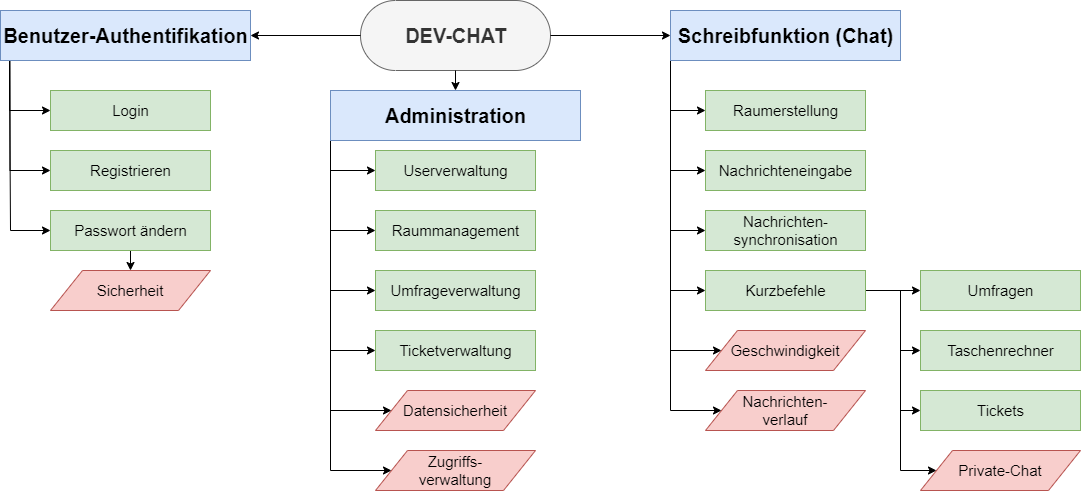
\includegraphics[width=1\textwidth, keepaspectratio]{images/Produktstruktur.png}
  \caption{Produktstruktur}
  \label{fig:Produktstruktur}
\end{figure}

\subsubsection{Benutzer-Authentifikation}\label{sec:BenutzerAuthentifikation}
Für die Authentifikation von Benutzern wird ein Login-System verwendet.
Dabei können sich Benutzer unter Angabe eines Benutzernamens, sowie Passworts registrieren und anmelden.
Für die Registrierung der Benutzer werden Kriterien definiert, welche sowohl die Sicherheit der Accounts, als auch die Benutzerfreundlichkeit gewährleisten sollen.

\noindent{}Für den Benutzernamen gelten deshalb die folgenden Kriterien:
\begin{itemize}
  \item Der Benutzername muss mindestens 4 und maximal 16 Zeichen lang sein
  \item Der Benutzername darf nur aus lateinischen Buchstaben und Zahlen bestehen
  \item Der Benutzername \gqq{admin} in jeglicher Groß- und Kleinschreibung steht nicht für Benutzer zur Verfügung, auch nicht als Teilwort eines Namens
\end{itemize}
Für das Passwort gelten die folgenden Kriterien:
\begin{itemize}
  \item Das Passwort muss mindestens 8 Zeichen lang sein
  \item Das Passwort muss mindestens einen Großbuchstaben, einen Kleinbuchstaben und eine Zahl enthalten
  \item Das Passwort darf nur aus lateinischen Buchstaben und Zahlen bestehen
\end{itemize} 
\noindent
Die Sicherheit der Passwörter wird durch die Verwendung von Hashwerten gewährleistet.
Das Passwort liegt somit nicht im Klartext, sondern als Hashwert in der Datenbank ab.
Während dem Anmeldeprozess wird das eingegebene Klartext-Passwort gehasht und mit dem in der Datenbank gespeicherten Hashwert verglichen.
Stimmen die Werte überein, wird der Benutzer eingeloggt.
Wird ein falsches Passwort eingegeben, wird der Benutzer durch das User Interface auf die Fehleingabe hingewiesen.
\newparagraph
Als Erweiterung des Login-Systems bietet \gqq{DEV-CHAT} die Möglichkeit, das eigene Passwort zu ändern.
Hierfür muss der Benutzer sowohl sein aktuelles Passwort, als auch das neue Passwort angeben.
Das neue Passwort muss dabei die oben genannten Kriterien erfüllen.

\subsubsection{Schreibfunktion}
Neben der Benutzer-Authentifikation bietet das Produkt die Möglichkeit, einen Chatraum zu erstellen oder einem bestehenden Chatraum beizutreten.
Bei der Erstellung eines Raumes, wird ein neuer Raumname generiert, welcher in dem User Interface angezeigt wird und für die anderen Nutzer als Zugangscode dient.
Dieser setzt sich dabei aus drei zufällig ausgewählten englischen Wörtern zusammen.
\newparagraph
Die Gültigkeit des Zugangscodes und damit auch des Chatraums ist standardmäßig auf einen Tag begrenzt.
In diesem Zeitraum können Nachrichten mit anderen Personen in dem erstellten Chatraum ausgetauscht werden.
Die gesendeten Nachrichten werden in einer Datenbank gespeichert, wodurch jedem Chat-Teilnehmer der gesamte Nachrichtenverlauf angezeigt werden kann.
Mit dem Ablauf der Gültigkeit des Zugangscodes werden aus Sicherheits- sowie Speicherplatzgründen alle Nachrichten aus der Datenbank gelöscht.
\newparagraph
Mittels einer aktiven Socket-Verbindung zwischen Client und Server wird sichergestellt, dass gesendete Nachrichten in Echtzeit mit allen anderen Benutzern synchronisiert werden.
Dank dieser Technik entfallen zyklische Abfragen des Servers, wodurch die Performance der Applikation verbessert wird.
\newparagraph
Neben der klassischen Schreibfunktion bietet \gqq{DEV-CHAT} auch die Möglichkeit, Kurzbefehle zu verwenden.
Alle zur Verfügung stehenden Befehle sind in Tabelle~\ref{tab:Kurzbefehle} aufgelistet und beziehen sich ausschließlich auf den Raum, in dem sie ausgeführt werden.

\begin{table}[H]
  \centering
  \begin{tabular}{|l|m{.5\linewidth}|m{.32\linewidth}|}
    \hline
    \textbf{Befehl} & \textbf{Beschreibung} & \textbf{Parameter} \\
    \hline
    /help     & Gibt alle Kurzbefehle aus                           & - \\
    \hline
    /calc     & Führt eine einfache Rechnung durch                  & Rechnung \\
    \hline
    /whisper  & Sendet eine Nachricht an einen bestimmten Benutzer  & Benutzername, Nachricht \\
    \hline
    /survey   & Erstellt eine Umfrage                               & Titel, Beschreibung, Antwortmöglichkeiten, Zeitdauer \\
    \hline
    /vote     & Abstimmen einer Umfrage                             & UmfrageID, AntwortID \\
    \hline
    /ticket   & Einsenden eines Fehlers                             & Fehlerbeschreibung \\
    \hline
  \end{tabular}
  \caption{Kurzbefehle}
  \label{tab:Kurzbefehle}
\end{table}
\noindent

\subsubsection{Administration}
Für die Moderation und Verwaltung des \gqq{DEV-CHAT} werden die Benutzer in zwei Rollen eingeteilt.
Standard-Benutzer sind in der Lage die in den vorherigen beiden Abschnitten beschriebenen Funktionen zu nutzen.
Administratoren hingegen sind in der Lage weitere Aktionen auszuführen.
Sie sind in erster Linie zuständig für die Verwaltung der Benutzer und Chat-Räume.
Dazu bietet \gqq{DEV-CHAT} eine grafische Administrationsoberfläche, welche durch die Rolle \gqq{Admin} freigeschaltet wird.
\newparagraph
Innerhalb dieser Administrationsoberfläche können folgende Aktionen durchgeführt werden:
Benutzer löschen, Passwörter auf ein Standard Passwort zurücksetzen, Rollen ändern (\gqq{Standard} oder \gqq{Admin}), Chat-Räume mit einem bestimmten Namen erstellen, Chat-Räume löschen, das Ablaufdatum eines Chatraums ändern, Umfragen löschen, das Ablaufdatum einer Umfrage ändern, erstellte Tickets einsehen und deren Status ändern (\gqq{To Do} oder \gqq{Done}).

\subsection{Merkmale der Qualität}\label{sec:ProduktUndGebrauchsqualitaet}
\subsubsection{Funktionalität (Kurzform)}
%//TODO: @Johannes @Lukas - Bitte noch mal drüber schauen!
% Im Prinzip eine Wiederholung des vorangehenden Kapitels -> Wird das nochmal benötigt?
\begin{itemize}
  \item Benutzer-Authentifikation
  \begin{itemize}
    \item Benutzer registrieren
    \begin{itemize}
      \item Benutzername, Password, Confirm Password eingeben
      \newline 
      → Müssen die Kriterien erfüllen
    \end{itemize}
    \item Benutzer löschen
    \newline
    → Alle zugehörigen Daten (Chat Nachrichten, Umfragen etc.) werden gelöscht
    \item Benutzer anmelden
    \newline
    → Benutzername und Passwort eingeben
    \item Benutzer abmelden
    \newline
    → Benutzer wird ausgeloggt
    \item Benutzer Passwort ändern
    \begin{itemize}
      \item Altes und neues Passwort eingeben
      \newline
      → Das neue Passwort muss die Kriterien erfüllen
    \end{itemize}
  \end{itemize}
  \item Schreibfunktion (Chat)
    \begin{itemize}
      \item Chatraum erstellen
      \newline
      → Der Raumname wird aus drei englischen Wörtern zufällig generiert und man wird nach der Erstellung direkt in den Chat weitergeleitet
      \item Chatraum beitreten
      \newline
      → Beitreten des gewünschten Chatraums
      \item Nachrichten senden
      \newline
      → Nachrichten können in den aktuellen Chatraum gesendet werden
      \item Nachrichten empfangen
      \newline
      → Alle Benutzer im aktuellen Chatraum können Nachrichten synchron empfangen
      \item Nachrichtenverlauf anzeigen
      \newline
      → Alle Nachrichten des aktuellen Chatraums werden angezeigt
      \item Kurzbefehle verwenden
      \begin{itemize}
        \item \gqq{/help}
        \newline
        → Zeigt eine Liste mit allen Kurzbefehlen an
        \item \gqq{/survey}
        \newline
        → Erstellt eine Umfrage mit den folgenden Parametern:
        \begin{itemize}
          \item Titel
          \item Beschreibung
          \item Antwortmöglichkeiten
          \item Zeitdauer
        \end{itemize}
        \item \gqq{/calc} 
        \newline
        → Bietet die Möglichkeit, eine einfache Rechnung durchzuführen
        \item \gqq{/whisper} 
        \newline
        → Sendet eine Nachricht an einen bestimmten Benutzer
        \item \gqq{/ticket} 
        \newline
        → Einsenden eines Fehlers
        \item \gqq{/vote}
        \newline
        → Abstimmen einer Umfrage mit einer Antwortmöglichkeit mit dem folgenden Parameter:
        \begin{itemize}
          \item UmfrageID
          \item AntwortID
        \end{itemize}
    \end{itemize}
  \end{itemize}
  \item Administration
    \begin{itemize}
      \item Benutzer verwalten
      \begin{itemize}
        \item Benutzer anzeigen
        \newline
        → Alle Benutzer werden tabellarisch angezeigt
        \item Benutzer löschen
        \newline
        → Alle zugehörigen Daten (Chat Nachrichten, Umfragen, etc.)werden gelöscht
        \item Benutzer Passwort zurücksetzen
        \newline
        → Das Passwort wird auf den Namen des Benutzers zurückgesetzt
        \item Benutzer Berechtigungsstatus ändern
        \newline
        → Der Benutzer erhält die Rolle \gqq{Admin} oder \gqq{Standard}
      \end{itemize}
    \item Chat-Räume verwalten
      \begin{itemize}
        \item Chat-Räume anzeigen
        \newline
        → Alle Chat-Räume werden tabellarisch angezeigt
        \item Custom-Chatraum erstellen
        \newline
        → Es kann ein Custom-Chatraum mit einem gewünschten Namen erstellt werden
        \item Custom-Chatraum löschen
        \newline
        → Es können Chat-Räume gelöscht werden
        \item Ablaufdatum eines Chatraums ändern
        \newline
        → Es kann das Ablaufdatum eines Chatraums geändert werden
      \end{itemize}
    \item Umfragen verwalten
      \begin{itemize}
        \item Umfragen anzeigen
        \newline
        → Alle Umfragen werden tabellarisch angezeigt
        \item Umfragen löschen
        \newline
        → Es können Umfragen gelöscht werden
        \item Ablaufdatum einer Umfrage ändern
        \newline
        → Es kann das Ablaufdatum einer Umfrage geändert werden
      \end{itemize}
    \item Tickets verwalten
      \begin{itemize}
        \item Tickets anzeigen
        \newline
        → Alle Tickets werden tabellarisch angezeigt
        \item Tickets löschen
        \newline
        → Es können Tickets gelöscht werden
        \item Tickets bearbeiten
        \newline
        → Es kann der Status eines Tickets geändert werden
      \end{itemize}  
    \end{itemize}   
\end{itemize}

\subsubsection{Effizienz}
Die Web-Applikation agiert bei allen Benutzerinteraktionen schnell und enthält keine Verzögerungen, die durch die Verarbeitung von Daten entstehen. 
Durch die Synchronisation der Chat-Räume bei allen Benutzern, wird die Performance nicht beeinträchtigt.

\subsubsection{Kompatabilität}\label{sec:Kompatibilitaet}
Die Web-Applikation \gqq{DEV-CHAT} ist mit allen gängigen Browsern kompatibel.
Dabei wurden insbesondere die Browser \gqq{Google Chrome}, \gqq{Mozilla Firefox} und \gqq{Microsoft Edge} getestet.
Durch die Entwicklung des User-Interface nach dem Prinzip \gqq{Mobile First} ist die Applikation sowohl für die Nutzung mit mobilen Endgeräten, als auch mit Desktop-Computern optimiert.

\subsubsection{Benutzbarkeit}
Der Intuitive Name \gqq{DEV-CHAT} indiziert, dass es sich bei der Applikation um ein Chat-System handelt.
Die Website setzt allgemein auf ein schlichtes Design, wobei die Hauptfunktionalitäten der Applikation in den Vordergrund gestellt werden.
Beim Betreten der Seite wird der Benutzer beispielsweise aufgefordert, sich anzumelden.
Analog zu anderen Web-Applikationen bietet die Applikation ebenfalls einen Verweis auf die Registrierung.
Neben dem Login Formular wird dem Benutzer zusätzlich ein Verweis zu einem \gqq{Getting Started} Guide angezeigt.
Dieser stellt dem Benutzer die Benutzeroberfläche, sowie die wichtigsten Funktionen der Applikation vor.
\newparagraph
Durch den begrenzten Funktionsumfang der Applikation ist die Benutzung intuitiv und selbsterklärend.
Gleichzeitig wird der Benutzer durch die Anzeige von Fehlermeldungen bei falschen Eingaben unterstützt.
Dadurch ist die Applikation für alle Benutzer geeignet.

\subsubsection{Zuverlässigkeit}
% Eine Software muss ein vorher definiertes Leistungsniveau über einen vorher definierten Zeitraum unter bestimmten Bedingungen halten können, um als zuverlässig zu gelten
Durch die Client Server Architektur der Applikation muss die Zuverlässigkeit sowohl für das Frontend, als auch für das Backend gewährleistet sein.
Die Zuverlässigkeit des Backends hängt dabei grundsätzlich von drei Faktoren ab: dem Code, der Hardware und den verwendeten externen Systemen.
Für die Zuverlässigkeit der Hardware sowie der externen Systeme müssen Anbieter und Technologien gewählt werden, die eine hohe Zuverlässigkeit garantieren.
Im Falle des \gqq{DEV-CHAT} wurde auf \gqq{Supabase} als Datenbank-Provider zurückgegriffen, welche sich neben einer hohen Zuverlässigkeit vor allem auch durch ihre kostenlosen Angebote auszeichnet.
Für den Betrieb des Backends wird auf eine eigene Hardware zurückgegriffen.
Dadurch muss die Zuverlässigkeit durch uns gewährleistet werden.
Die Zuverlässigkeit des Codes kann beispielsweise durch Unit-Tests und Integrationstests sichergestellt werden.
Aufgrund der begrenzten Ressourcen wurde bislang auf die Verwendung von Unit- und Integrationstests verzichtet.
\newparagraph
Für die Zuverlässigkeit des Frontends beschränkt sich der Einflussbereich während der Entwicklung auf den Code, sowie das \ac{API} des Backends, da Faktoren wie die verwendete Hardware oder der verwendete Browser nicht durch die Entwickler beeinflusst werden können.
Auch hier können für die Zuverlässigkeit des Codes beispielsweise Unit-Tests und Integrationstests verwendet werden.

\subsubsection{Sicherheit}
% Passwort Hashing
% Standard Berechtigung -> keine Admin Funktionen
% Sicherheitsabfragen im Backend -> User-Validation, SQL-Injection, XSS
% SSL
Um die Sicherheit der Daten und damit der Website zu gewährleisten, werden verschiedene Sicherheitsmaßnahmen umgesetzt.
Zunächst wird für die Kommunikation zwischen Client und Server das Protokoll \ac{HTTPS} verwendet, wodurch sämtliche Übertragungen mittels dem \ac{SSL}-Verfahren verschlüsselt werden.
Dies ermöglicht unter anderem die sichere Übertragung der Klartext Passwörter während des Login-Prozesses.
Um die Sicherheit der Passwörter in der Datenbank zu gewährleisten, werden diese wie bereits in Kapitel~\ref{sec:BenutzerAuthentifikation} beschrieben als Hashwert gespeichert.
\newparagraph
Um den Zugriff auf Bereiche der Web-Applikation für nicht autorisierte Benutzer zu verhindern, wird bei der Erstellung eines neuen Benutzers die Berechtigung \gqq{Standard} zugewiesen.
Für alle Zugriffe auf Funktionen der Applikation, welche nur durch eingeloggte Benutzer ausgeführt werden dürfen, überprüft das Backend des Systems zunächst den Login Status des Benutzers.
Für den Zugriff auf besondere Bereiche wie etwa der Administrationsoberfläche wird zusätzlich die Berechtigung des Benutzers geprüft.
\newparagraph
Erlaubt die Weboberfläche dem Benutzer die Eingabe von Text, welcher anschließend an das Backend übertragen wird, so werden die Eingaben zunächst vom Backend validiert.
Dadurch können Angriffe wie \ac{SQL}-Injections oder \ac{XSS} verhindert werden.

\subsubsection{Wartbarkeit}
% Modularität durch Klassen
% Bsp.: Kurzbefehle als Klassen-Struktur -> Erweiterung durch neue Klasse
% Trennung zwischen Frontend und Backend
Für die Umsetzung der Web-Applikation wurde das Framework Next.js verwendet, welches neben der Entwicklung von UI Komponenten basierend auf React, auch ein Backend mittels Node.js bereitstellt.
Dabei wird durch die Projektstruktur eine klare Trennung zwischen Frontend und Backend sichergestellt.
\newparagraph
Im Rahmen des \gqq{DEV-CHAT} wurde auf eine objektorientierte Programmierung mit der Verwendung von klassenbasierten Komponenten gesetzt.
Dadurch wird eine modulare Struktur der Applikation erreicht.
Diese sorgt für eine unkomplizierte Erweiterbarkeit der Applikation, welche besonders an dem Beispiel der Kurzbefehle deutlich wird.
Die Kurzbefehle sind in ihrer Struktur durch eine Oberklasse definiert.
Abgeleitet von der Oberklasse werden die einzelnen Kurzbefehle implementiert, wodurch für eine Erweiterung der Kurzbefehle lediglich eine neue Unterklasse angelegt werden muss.
\newparagraph
Durch die Unterteilung der Applikation in mehrere Module (Klassen) wird außerdem die Testbarkeit der Applikation erleichtert.

\subsubsection{Übertragbarkeit}
Durch die Verwendung einer Web-Applikation ist die Übertragbarkeit der Applikation in einem hohen Umfang gegeben.
Dies lässt sich dadurch begründen, dass Webbrowser auf allen gängigen Betriebssystemen zur Verfügung stehen, wodurch eine Betriebssystemunabhängigkeit erreicht wird.
Gleichzeitig stehen Webbrowser sowohl auf mobilen, als auch auf stationären Endgeräten zur Verfügung.
Durch die adaptive Entwicklung der Benutzeroberfläche, wie in Kapitel~\ref{sec:Kompatibilitaet} beschreiben, lässt sich die Anwendung somit auf allen gängigen Endgeräten ohne Einschränkungen der Benutzerfreundlichkeit nutzen.

\subsection{Nutzererwartungen}
Die Erwartungen von Nutzern an ein Softwareprodukt lassen sich grundsätzlich in die drei Kategorien verborgene Erwartungen, prägende Erwartungen und kognitive Erwartungen unterteilen.
Diese Kategorien werden in den folgenden Unterkapiteln näher erläutert.

\subsubsection{Verborgene Erwartungen}
Verborgene Erwartungen sind unbewusst und entstehen durch die Erfahrungen, die der Nutzer mit anderen Produkten gemacht hat.
Dazu zählen zum Beispiel bestimmte Interaktionsmuster, Navigationsarten, Layouts und Designs.
Beispielsweise wird bei den meisten Desktop-Applikationen erwartet, dass diese üblicherweise an der oberen rechten Seite mit einem Button geschlossen werden können.
Ein weiteres Beispiel, welches ebenfalls im Kontext \gqq{DEV-CHAT} relevant ist, ist die Unabhängigkeit der Applikation von dem Betriebssystem, beziehungsweise der Art der zugrundeliegenden Hardware.

\subsubsection{Prägende Erwartungen}
Prägende Erwartungen ergeben sich aus der Erfahrungen mit der Benutzung bestimmter Applikationen.
Bestimmte Interaktionsmuster oder auch Designentscheidungen werden durch eine regelmäßige Benutzung verinnerlicht und als intuitiv empfunden.
Ein Beispiel hierfür ist Social Media.
Die meisten Nutzer sind mit der Benutzung von Social-Media-Plattformen vertraut und kennen den Sinn und Zweck der enthaltenen Interaktionselemente.
Bei der Entwicklung einer neuen Anwendung, wird somit erwartet, dass diese Elemente ebenfalls vorhanden sind.

\subsubsection{Aktuelle Erwartungen}
Aktuelle Erwartungen sind bewusste Erfahrung, welche mit der aktuellen Situation verbunden sind.
Nutzer sind bewusst auf einer Website und verfolgen ein bestimmtes, bekanntes Ziel. 
Gibt es einen Bruch in der Erwartung, wird die Nutzerreaktion negativ sein. 
Die natürliche Nutzerreaktion ist das Verlassen der Applikation \autocite{noauthor_user_nodate}.

\subsection{Akzeptanzkriterien}
Akzeptanzkriterien beschreiben, wann eine bestimmte Anforderung in einem Entwicklungsteam als abgeschlossen gelten kann.
Hierbei ist zu beachten, dass diese objektiv und eindeutig zu überprüfen sind, damit alle Erwartungen wie gewollt umgesetzt worden sind \autocite{noauthor_akzeptanzkriterien_nodate}.

\subsection{Technisch wenig versierter Nutzer}
% verfügt nicht über nötige Kenntnisse zur intuitiven Nutzung der Applikation
% Keine Ahnung von z.B. Kurzbefehlen
% Ohne Anleitung nicht in der Lage die Applikation zu nutzen -> verlässt die Applikation
% Keine großen Anforderungen an die Geschwindigkeit
% Admin Rechte -> Kritisch -> Unbefugter Zugriff, unkontrollierte Verwaltung der Applikation -> Sicherheitsrisiko
Ein technisch wenig versierter Nutzer verfügt nicht über die nötigen Kenntnisse, um die Applikation intuitiv zu nutzen.
Aus diesem Grund erwartet er eine detaillierte Anleitung zur Nutzung der Applikation.
Basierend auf der Anleitung erlernt er die grundlegenden Abläufe zur Erstellung eines Accounts und zum Betreten eines Chatraums.

\noindent{}Innerhalb des Chatraums erwartet der Nutzer lediglich die Chatfunktion.
Sämtliche weitere Funktionen, wie etwa die Verwendung von Kurzbefehlen, müssen durch die Anleitung erlernt werden.
Auch Anforderungen an die Geschwindigkeit der Applikation sind für den Nutzer nicht hoch priorisiert.

\noindent{}Die Vergabe der \gqq{Admin} Rolle an technisch wenig versierte Nutzer ist unter allen Umständen zu vermeiden, da dies ein Sicherheitsrisiko darstellt.
Über die Administrationsoberfläche erhält der Nutzer die Fähigkeit unbewusst Chat-Räume und Umfragen zu löschen oder Benutzer-Rollen zu vergeben und Passwörter zurückzusetzen.

\noindent{}Aus diesen Gründen ergeben sich die folgenden Nutzererwartungen und Akzeptanzkriterien.

\subsubsection{Nutzererwartungen}
% Anleitung/Tutorial/Erklärung
% Chatapplikation ohne großartige Zusatzfunktionen
\begin{itemize}
  \item Die Applikation ist möglichst ähnlich zu bekannten Chat-Applikationen aufgebaut (Prägende Erwartungen)
  \item Die Applikation bietet ausschließlich die Chat-Funktion (Aktuelle Erwartungen)
  \item Es gibt eine detaillierte/geführte Anleitung zur Nutzung der Applikation (Verborgene Erwartungen)
\end{itemize}

\subsubsection{Akzeptanzkriterien}
\begin{itemize}
  \item Es existiert eine (unkomplizierte) Anleitung für das entwickelte Feature
  \item Es ist möglich, einen Chatraum zu betreten und mit anderen Nutzern zu chatten
\end{itemize}

\subsection{Technisch versierter Nutzer}
% Besitzt Erfahrung mit der Benutzung von Chat-Applikationen
% Erwartet einfache, intuitive Bedienung + schnelle Reaktion
% Terminal-Style -> erwartet Befehle
% Admin -> Macht sich mit der Applikation vertraut -> nutzt die Funktionen nur wenn nötig
Im Gegensatz zu dem technisch wenig versierten Nutzer, kann der technisch versierte Nutzer auf Erfahrungen mit anderen Chat-Applikationen zurückgreifen.
Aus diesem Grund erwartet er eine einfache, intuitive Bedienung der Applikation, wobei besonders die Reaktionsgeschwindigkeit einen hohen Stellenwert einnimmt.
Zusätzlich erwartet er die für Chat-Applikationen üblichen Funktionen, wie die Unterteilung in verschiedene Chat-Räume und die Echtzeitkommunikation zwischen den Nutzern.
\newparagraph
Durch den Konsolen-Style des Chatraums erwartet der Nutzer ebenfalls die Möglichkeit, Befehle zu verwenden.
Der Befehl \gqq{/help} ist dabei ein weit verbreiteter Befehl um eine Liste aller verfügbaren Befehle anzuzeigen.
\newparagraph
Erhält der Nutzer die \gqq{Admin}-Rolle, so macht er sich zunächst mit der Administrationsoberfläche vertraut.
Da er sich bereits mit der Applikation auseinandergesetzt hat, weiß er wie er mit den bereitgestellten Funktionen umgehen muss.
Erhält er ungewollt die Rolle \gqq{Admin}, kann der technisch versierte Nutzer entweder verantwortungsvoll mit der Rolle umgehen oder gar zu einer noch größeren Gefahr als der technisch weniger versierte Nutzer werden.
Durch sein erweitertes Wissen über den Umgang mit der Applikation kann er gezielt Schaden anrichten, weshalb eine ungewollte Vergabe der Rolle ebenfalls zu vermeiden ist.

\subsubsection{Nutzererwartungen}
\begin{itemize}
  \item Aufbau und Features sind ähnlich zu bekannten Chat-Applikationen (Prägende Erwartungen)
  \item Durch den Konsolen-Style gibt es Befehle, die verwendet werden können (Prägende Erwartungen)
  \item Die Eingabe und Verarbeitung von Daten erfolgt ohne große Verzögerung (Verborgene Erwartungen)
  \item Es gibt eine Administrator-Rolle welche befugt ist, die Funktionen der Applikation zu verwalten (Verborgene Erwartungen)
  \item Die Chat Nachrichten werden mit Ende-zu-Ende-Verschlüsselung übertragen (Verborgene Erwartungen)
  \item Das Design der Applikation soll einem technisch versierten Nutzer bekannt vorkommen (Aktuelle Erwartungen)
\end{itemize}

\subsubsection{Akzeptanzkriterien}
\begin{itemize}
  \item Es existiert eine Anleitung für das entwickelte Feature
  \item Die Web-Applikation weist keine Performance Probleme auf
  \item Das Benutzer Passwort wird verschlüsselt gespeichert
\end{itemize}

\subsection{Spezifizieren einer Anforderungen in \gqq{halbformaler} Beschreibung}
Die Tabelle~\ref{tab:AnforderungBenutzerRegistrieren} zeigt die Anforderung \gqq{Benutzer registrieren} in \gqq{halbformaler} Beschreibung.
\begin{table}[H]
  \centering
  \resizebox{\columnwidth}{!}{%
  \begin{tabular}{|l|l|}
  \hline
  Beschreibung  & Anforderung                                          \\ \hline
  Funktion      & Benutzer registrieren                                \\ \hline
  Beschreibung  & Einen neuen Benutzer für den \gqq{DEV-CHAT} registrieren \\ \hline
  Eingaben &
    \begin{tabular}[c]{@{}l@{}}Benutzerdaten:\\ Benutzername, 2x Passwort (Das zweite Passwort für die Bestätigung)\end{tabular} \\ \hline
  Ausgaben      & -                                                    \\ \hline
  Abfolge &
    \begin{tabular}[c]{@{}l@{}}Nutzer öffnet die Web-Applikation \gqq{DEV-CHAT}\\ Klicken des Hyperlinks \gqq{create Account}\\ Benutzername eingeben\\ Passwort eingeben\\ Confirm Passwort eingeben\\ Klicken des Buttons \gqq{Create}\end{tabular} \\ \hline
  Ausnahmen     & Benutzername existiert bereits                       \\ \hline
  Vorbedingung  & -                                                    \\ \hline
  Nachbedingung & Benutzer wird nach der Erstellung direkt eingeloggt  \\ \hline
  Einschränkung &
    \begin{tabular}[c]{@{}l@{}}Benutzername entspricht nicht den Richtlinien\\ Passwort entspricht nicht den Richtlinien\\ Confirm Passwort stimmt nicht mit dem Passwort überein\end{tabular}
  \\ \hline
  \end{tabular}%
  }
  \caption{Anforderung: Benutzer registrieren}
  \label{tab:AnforderungBenutzerRegistrieren}
\end{table}

  \section{Fehler, Kosten und Qualitätsmaßnahmen}

% kurze Einleitung zum Thema




\subsection{Beschreiben Sie typische Faults and Defects Ihres Software-Produkts. Stellen Sie Fehlerschwere, Priorität und potentielle Fehlerkosten dar.}

% Notizen: 
    % Error: Fehlhandlung (Menschliche Handlung die zu einem nicht korrektem Resultat führt Beispiel: Programmierer – Fehler in Programmcode.)
    % Fault: Fehlerzustand (Auftreten eines Fehlers in der Software.)
    % Failure (/Defect): Fehlerwirkung (Bei der Programmausführung kommt es zu einem Abbruch  oder bestimmte Funktionen können nicht wie spezifiziert ausgeführt werden.)

% Aufgaben Aufbau:
    % Faults und Defects [] (-> Tabelle?)
        % Fehlerschwere (1-5) (Prio auch noch mit rein?)
        % Priorität
        % potentielle Fehlerkosten




\subsection{Stellen Sie dar, wie sie die Q-Kosten in der Entwicklung des Produktes senken können? Warum ist es nicht sinnvoll komplette Fehlerfreiheit anzustreben und nennen Sie Methoden und Modelle aus der Vorlesung, die zum Einsatz kommen könnten?}

% Wie Entwicklungskosten senken?

% Warum nicht komplette Fehlerfreiheit?

% Methoden aus der Vorlesung um Entwicklungskosten zu senken




\subsection{Führen Sie eine FMEA für Ihr Produkt durch – für die RPZ treffen Sie realistische Annahmen}

% Failure Mode and Effects Analysis (FMEA) (realistische Annahme für Risikoprioritätszahl RPZ





  \include{chapter/FehlerKostenQualitaetsmaßnahmen.tex}

  %%%%%%%%%%%%%%%%%%%%%%% Literaturverzeichnis %%%%%%%%%%%%%%%%%%%%%%%
  \phantomsection
\addcontentsline{toc}{section}{Literatur}
\printbibliography
\newpage


  %%%%%%%%%%%%%%%%%%%%%%%%%%%%%% Anhang %%%%%%%%%%%%%%%%%%%%%%%%%%%%%%
  \renewcommand{\thetable}{\Alph{section}.\arabic{table}}
  \renewcommand{\thefigure}{\Alph{section}.\arabic{figure}}
  \renewcommand{\thelstlisting}{\Alph{section}.\arabic{lstlisting}}
  \pagenumbering{Alph}

  \begin{appendix}
  \section{Anhang}
\end{appendix}
\end{document}